\documentclass[glossy]{beamer}
\useoutertheme{wuerzburg}
\useinnertheme[realshadow,corners=2pt,padding=2pt]{chamfered}
\usecolortheme{shark}

\usepackage{listings}

\usepackage{fancyvrb}
%\usepackage[scaled]{beramono} %sets the beramono font. Just comment this line to get the default font back

\usepackage{tikz}
\newcommand<>{\hover}[1]{\uncover#2{%
 \begin{tikzpicture}[remember picture,overlay]%
 \draw[fill,opacity=0.4] (current page.south west)
 rectangle (current page.north east);
 \node at (current page.center) {#1};
 \end{tikzpicture}}
}

\title{Arquitecturas y Organización de Computadoras I \\\line(1,0){320}}
% \author{\texorpdfstring{Author\newline\url{email@email.com}}{Author}}
%\author{Rafael Ignacio Zurita}
\institute{Rafael Ignacio Zurita \\ Departamento de Ingenieria de Computadoras - FAI - UNCOMA 2018 \\ Clase presencial 4}
%\date{\today}



\begin{document}




\begin{frame}
\maketitle
\end{frame}

\institute{Departamento de Ingenieria de Computadoras - FAI - UNCOMA \\ 2018}

\begin{frame}
\frametitle{Programa Analítico}
\textbf{UNIDAD I: Arquitectura y Organización de Computadoras}
 \\~\\
\textit{Formatos de instrucciones. Modos de direccionamiento. Tipos de instrucciones. Lenguaje ensamblador: directivas, operaciones, pseudo-operaciones, macros.} 
 \\~\\
\end{frame}


\begin{frame}
\frametitle{Temario}
\begin{itemize}
\item Operaciones (instrucciones) y el conjunto de instrucciones MIPS
\item Modos de direccionamiento
\item Lenguaje Máquina
\item Ensamblador
\item Traducción de declaraciones en C a lenguaje ensamblador
\end{itemize}
\end{frame}



\begin{frame}
\frametitle{Tipos de Instrucciones}
\begin{center}\textbf{Tipos Principales de Instrucciones}\end{center}
\begin{itemize}
\item Aritméticas
\begin{itemize}
\item Enteros
\item Punto Flotante
\end{itemize}
\item Instrucciones de transferencia de datos (memoria)
\begin{itemize}
\item Carga y Almacenamiento
\end{itemize}
\item Flujo de control
\begin{itemize}
\item Salto
\item Bifurcación condicional
\item Llamado y Retorno
\end{itemize}
\end{itemize}
\end{frame}



\begin{frame}[fragile]
\frametitle{Tipos de Instrucciones}
\begin{center}\textbf{Instrucciones aritméticas en MIPS}\end{center}
\begin{itemize}
\item Las instrucciones aritméticas lógicas más comunes tienen 3 operandos
\item El orden de los operandos es fijo (el destino primero)
\item Ejemplo:
\end{itemize}

% \footnotesize
\begin{verbatim}

  Código C:        a = b + c;

  Código MIPS:     add s0, s1, s2

(el compilador asocia a s0, s1 y s2 a las variables a, b y c)

\end{verbatim}

\end{frame}



\begin{frame}[fragile]
\frametitle{Tipos de Instrucciones}
\begin{center}\textbf{Instrucciones aritméticas en MIPS}\end{center}

\begin{verbatim}

  Código C:        a = b + c + d;
                   e = f - a;

  Código MIPS:     add $t0, $s1, $s2
                   add $s0, $t0, $s3
                   sub $s4, $s5, $s0
\end{verbatim}
\begin{itemize}
\item Los operandos deben estar en registros, y existen sólo 32
\item Principio de diseño: Más pequeño es más rápido. Porqué? (viaje de las señales)
\end{itemize}
\end{frame}





\begin{frame}
\frametitle{Tipos de instrucciones en MIPS}
\begin{center}\textbf{Registros vs. Memoria}\end{center}

\begin{itemize}
\item Los operandos deben estar en registros, y existen sólo 32
\item El compilador asocia variables a registros
\item ¿Qué sucede con un programa con un montón de variables?
\end{itemize}
\begin{center}
\begin{figure}
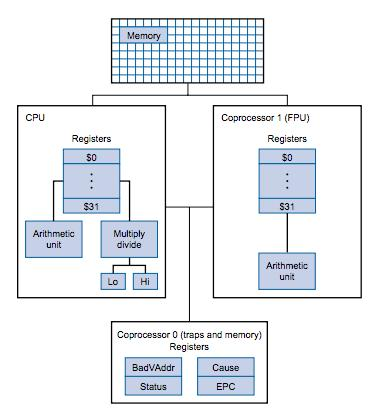
\includegraphics[scale=0.4]{organizacion-mips.jpg} 
\end{figure}
\end{center}
\end{frame}


\begin{frame}
\frametitle{Representación de datos a nivel máquina}
\textbf{Organización de la Memoria principal en MIPS}
\begin{itemize}
	\item $2^{32}$ bytes, con direcciones 0, 1, 2 ... 
	\item $2^{30}$ 4-bytes palabras, con direcciones 0, 4, 8 ... 
	\item Las direcciones de las palabras deben ser múltiplos de 4
\end{itemize}
	\begin{center}
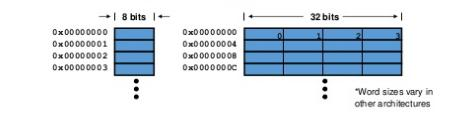
\includegraphics[scale=0.5]{memoria-mips.jpg} 
	\end{center}
\end{frame}


\begin{frame}[fragile]
\frametitle{Tipos de Instrucciones}
\begin{center}\textbf{Registros vs. Memoria}\end{center}

\begin{itemize}
\item Los operandos deben estar en registros, y existen sólo 32
\item El compilador asocia variables a registros
\item ¿Qué sucede con un programa con un montón de variables?
\end{itemize}
\end{frame}



\begin{frame}[fragile]
\frametitle{Tipos de Instrucciones}
\begin{center}\textbf{Asignación de Registros}\end{center}

\begin{itemize}
\item El compilador intenta asociar tantas variables a registros como sea posible
\item Algunas variables no pueden ser alocadas
\begin{itemize}
\item grandes arreglos (vectores)
\item variables accedidas con diferentes punteros
\item variables alocadas dinamicamente
\begin{itemize}
\item heap
\item stack
\end{itemize}
\end{itemize}
\end{itemize}
\end{frame}



\begin{frame}
\frametitle{Programación de la máquina: lenguaje ensamblador MIPS}
        \begin{center}
        \textbf{Conjunto básico de instrucciones MIPS}
        \end{center}
\begin{tabular}{cl}

\begin{tabular}{c}
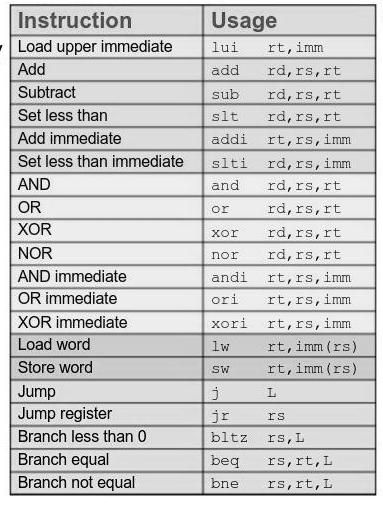
\includegraphics[height=5cm, width=4cm]{instrucciones-mips.jpg}

\end{tabular}
& \begin{tabular}{l}
\parbox{0.5\linewidth}{

%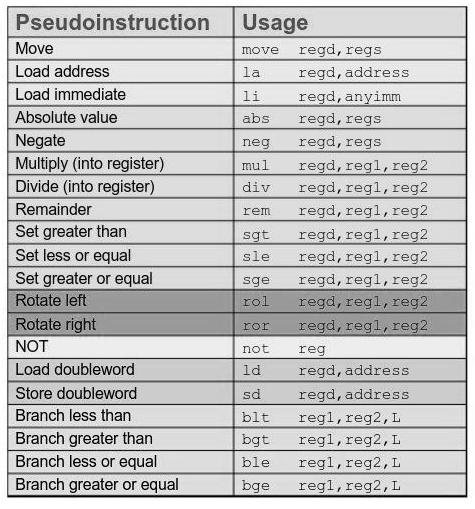
\includegraphics[height=5.2cm, width=4cm]{pseudoinstrucciones-mips2.jpg}
}
\end{tabular} \\

\end{tabular}
\end{frame}


\begin{frame}
\frametitle{Formato de  instrucciones en MIPS}
	\textbf{3 Formatos (fácil decodificación en hardware)}
	\begin{center}
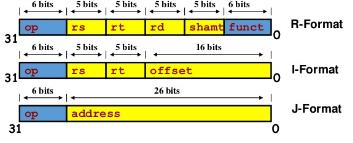
\includegraphics[scale=0.5]{formato.jpg} 
	\end{center}
\end{frame}


\begin{frame}
\frametitle{Formato de instrucciones en MIPS}
	\textbf{Un ejemplo completo de traducción al lenguaje de la máquina}
	\begin{center}
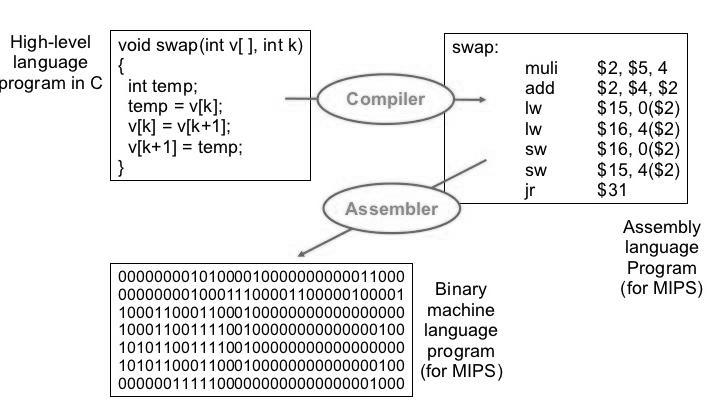
\includegraphics[scale=0.4]{below2.jpg} 
	\end{center}
\end{frame}


\begin{frame}
 \frametitle{Consejos y preguntas}
\begin{center}
\begin{itemize}
\item  ¿Preguntas?
\end{itemize}
\end{center}
\end{frame}


\begin{frame}
 \frametitle{Bibliografía}
Libros
\begin{itemize}
\item Andrew S. Tanenbaum (2000), ORGANIZACIÓN DE COMPUTADORAS un enfoque estructurado, Editorial Prentice Hall. (10 copias en biblioteca)
\item David. Patterson John L. Hennessy (1995), ORGANIZACIÓN Y DISEÑO DE COMPUTADORES La interfaz hardware/software, McGraw-Hill (8 copias en biblioteca).
\end{itemize}
Contenido electrónico
\begin{itemize}
	\item \textbf{x86 assembly basis} Una introducción al lenguaje ensamblador x86. Disponible en PEDCO en formato PDF.
		\url{https://www.nayuki.io/page/a-fundamental-introduction-to-x86-assembly-programming}
\item Apuntes elaborados por la cátedra, disponibles en PEDCO para impresión (pdf) o lectura online (html)
\item Secciones de libros aptas para publicacion
\end{itemize}
\end{frame}


\end{document}
